%!TEX root = doc.tex
\documentclass[twoside,10pt,parskip=half,ngerman]{scrreprt}

%***********************************************************************
% include some libs
%***********************************************************************
\usepackage[utf8]{inputenc}
\usepackage{listings}
\usepackage{xcolor}
\usepackage{color}
\usepackage{fancyhdr}
\usepackage{rotating}
\usepackage{titlesec}
\usepackage{mathptmx}
\usepackage{amssymb} % checkmark
% \usepackage{helvet}
\usepackage[scaled]{uarial}
\renewcommand*\familydefault{\sfdefault} %% Only if the base font of the document is to be sans serif
\usepackage[T1]{fontenc}
\usepackage[ngerman]{babel}
\usepackage[pdfauthor={Nicolas Roos}, pdftitle={Projektarbeit im Seminar Mobile Netzwerke - Wifi basierte Aktionen (Android App)}, colorlinks=true,linkcolor=black,citecolor=black,plainpages=false]{hyperref}
\usepackage{textcomp}
\usepackage[squaren]{SIunits}
\usepackage{graphicx}
\usepackage{url}
\usepackage{geometry}
\usepackage[absolute]{textpos}
\usepackage{makeidx}
\usepackage{colortbl}
\usepackage{pdflscape}
\usepackage{pdfpages}
\usepackage{tabularx}
\usepackage{lmodern}
\usepackage{longtable}
\usepackage{array}
\usepackage{float}
\usepackage{scrhack}
\usepackage{wallpaper} %\ThisTileWallPaper{}
\usepackage[super,square]{natbib} %für BibTeX Literaturverzeichnis
\usepackage{packages/usecases}
% Glossar
\usepackage{footnote}
\makesavenoteenv{description}
\usepackage[acronym,section=section]{glossaries}
\renewcommand*{\glsentryfmt}{\ifglsused{\glslabel}{\glsentryname{\glslabel}}{\glsentrydesc{\glslabel}\space(\glsentryname{\glslabel})}}
\makeglossaries

%***********************************************************************
% various styles
%***********************************************************************

%create index
\makeindex

%define pagestyle
\pagestyle{fancy}

%use sans-serif font
%\renewcommand{\familydefault}{\sfdefault}

%define page margin
\geometry{a4paper, top=30mm, left=30mm, right=30mm, bottom=30mm,headsep=10mm,footskip=10mm}

%textpos parameter
\setlength{\TPHorizModule}{30mm}
\setlength{\TPVertModule}{\TPHorizModule}
\textblockorigin{10mm}{10mm} % start everything near the top-left corner
\setlength{\parindent}{0pt}

%horizontal lines for titlepage
\newcommand{\HRule}{\rule{\linewidth}{0.5mm}}

%reference to source items inlc source number
\newcommand{\srcref}[1]{\nameref{src:#1} \cite{#1}}

%header / footer
\renewcommand{\headrulewidth}{0.3pt}
\renewcommand{\footrulewidth}{0.3pt}

\fancyhead[LO,RE]{} %clear headings for contents
\fancyhead[RO,LE]{\nouppercase{\rightmark}} %right odd pages and left even pages
\fancyhead[LO,RE]{\MakeUppercase{\leftmark}} %left odd pages and right even pages
\fancyfoot[LE,RO]{\thepage} %page numbering
\fancyfoot[C]{} %clear centered page numbering

%define some colors
\definecolor{gray}{rgb}{0.95,0.95,0.95}
\definecolor{darkgray}{rgb}{0.4,0.4,0.4}
%listing colors
\definecolor{lgray}{RGB}{250,250,250}
\definecolor{lgreen}{RGB}{63,127,95}
\definecolor{lred}{RGB}{127,0,85}
\definecolor{lblue}{RGB}{42,0,255}

%***********************************************************************
% listing
%***********************************************************************

\lstset{
		basicstyle=\small\ttfamily,
		frame=single,
		numbers=left,
		numberstyle=\tiny,
		%firstnumber=auto,
		numberblanklines=true,
		captionpos=b,
		extendedchars=true,
		float=ht,
		showtabs=false,
		tabsize=2,
		showspaces=false,
		showstringspaces=false,
		breaklines=true,
		%prebreak=\Righttorque,
		backgroundcolor=\color{lgray},
		keywordstyle=\color{lred}\bfseries,
		commentstyle=\color{lgreen}\ttfamily,
%		morekeywords={printstr, printhexln},
		stringstyle=\color{lblue},
		xleftmargin=0.5cm,
		xrightmargin=0.5cm
}

\lstloadlanguages{[Sharp]C}
%\lstdefinestyle{sharpc}{language=[Sharp]C, frame=lr} %, rulecolor=\color{blue!80!black}

%\lstdefinelanguage{xc}{
%     keywords={printstr, printhexln, attributes, class, classend, do, empty, endif, endwhile, fail, function, functionend, if, implements, in, inherit, inout, not, of, operations, out, return, set, then, types, while, use},
%     keywordstyle=\color{lred}\bfseries,
%     ndkeywords={},
%     ndkeywordstyle=\color{yellow}\bfseries,
%     identifierstyle=\color{black},
%     sensitive=false,
%     comment=[l]{//},
%     commentstyle=\color{lgreen}\ttfamily,
%     string=[l]{"},
%     stringstyle=\color{lblue}\ttfamily
%  }


\begin{document}
%!TEX root = ../doc.tex
\newglossaryentry{zhaw}{name=ZHAW,description=Zürcher Hochschule für Angewandte Wissenschaften}

\bibliographystyle{plainnat}

\title{Projektarbeit im Seminar Mobile Netzwerke - Wifi basierte Aktionen (Android App)} % In header.tex nachtragen
\author{Nicolas Roos}

%!TEX root = ../doc.tex
\begin{titlepage}

% Logo
\ThisTileWallPaper{\paperwidth}{\paperheight}{images/logos/SoE.pdf} % {images/logos/*.pdf}

\begin{minipage}[b]{0.117\textwidth}
\hskip 0.05cm
\end{minipage}
\begin{minipage}[b]{0.91\textwidth}
\begin{tiny}.\end{tiny}\vskip 2.8cm
	{\huge

	% Projekt Name (max. 2 Zeilen)
	\textbf{\underline{Bachelor-/Projektarbeit}}\\
	\textbf{\underline{FS14 Studiengang Informatik}}\\

	% Projekt Titel (max. 4 Zeilen)
	Titel der Arbeit
	\vskip 0.5cm}

	\begin{minipage}[b]{0.27\textwidth}
	\hrule\vskip 0.5cm
		\textbf{Autoren}\\
		\\
	\end{minipage}
	\begin{minipage}[b]{0.03\textwidth}
	\hskip 0.5cm
	\end{minipage}
	\begin{minipage}[b]{0.7\textwidth}
	\hrule\vskip 0.5cm
		Vorname Name\\
		Vorname Name\\
	\end{minipage}

	\begin{minipage}[b]{0.27\textwidth}
	\hrule\vskip 0.5cm
		\textbf{Hauptbetreuung}\\
		\\
	\end{minipage}
	\begin{minipage}[b]{0.03\textwidth}
	\hskip 0.5cm
	\end{minipage}
	\begin{minipage}[b]{0.7\textwidth}
	\hrule\vskip 0.5cm
		Vorname Name\\
		Vorname Name\\
	\end{minipage}

	\begin{minipage}[b]{0.27\textwidth}
	\hrule\vskip 0.5cm
		\textbf{Nebenbetreuung}\\
		\\
	\end{minipage}
	\begin{minipage}[b]{0.03\textwidth}
	\hskip 0.5cm
	\end{minipage}
	\begin{minipage}[b]{0.7\textwidth}
	\hrule\vskip 0.5cm
		Vorname Name\\
		Vorname Name\\
	\end{minipage}

	\begin{minipage}[b]{0.27\textwidth}
	\hrule\vskip 0.5cm
		\textbf{Industriepartner}\\
		\\
	\end{minipage}
	\begin{minipage}[b]{0.03\textwidth}
	\hskip 0.5cm
	\end{minipage}
	\begin{minipage}[b]{0.7\textwidth}
	\hrule\vskip 0.5cm
		Firmenname\\
		\\
	\end{minipage}

	\begin{minipage}[b]{0.27\textwidth}
	\hrule\vskip 0.5cm
		\textbf{Externe Betreuung}\\
		\\
	\end{minipage}
	\begin{minipage}[b]{0.03\textwidth}
	\hskip 0.5cm
	\end{minipage}
	\begin{minipage}[b]{0.7\textwidth}
	\hrule\vskip 0.5cm
		Vorname Name\\
		Vorname Name\\
	\end{minipage}

	\begin{minipage}[b]{0.27\textwidth}
	\hrule\vskip 0.5cm
		\textbf{Datum}
	\end{minipage}
	\begin{minipage}[b]{0.03\textwidth}
	\hskip 0.5cm
	\end{minipage}
	\begin{minipage}[b]{0.7\textwidth}
	\hrule\vskip 0.5cm
		\today
	\end{minipage}
\end{minipage}
\vskip 0.5cm


\textcolor{darkgray}{
Bitte füllen Sie das Titelblatt aus und berücksichtigen Sie Folgendes:\\
 -> Bitte auf keinen Fall Schriftart und Schriftgrösse ändern. Text soll lediglich überschrieben werden!\\
 -> Bitte pro Tabellenzeile max. 4 Textzeilen!\\
\\
•	Titel: Fügen Sie Ihren Studiengang direkt nach dem Wort „Bachelorarbeit“ ein (max. 2 Zeilen).\\
•	Titel der Arbeit: Überschreiben Sie den Lauftext mit dem Titel Ihrer Arbeit (max. 4 Zeilen).\\
•	Autoren: Tragen Sie Ihre Vor- und Nachnamen ein (alphabetisch nach Name).\\
•	Betreuer: Tragen Sie Ihren Betreuer / Ihre Betreuer ein (alphabetisch nach Name).\\
•	Ohne Nebenbetreuung, Industriepartner oder externe Betreuung, ganze Tabellenzeile löschen.\\
•	Am Schluss löschen Sie den ganzen Beschrieb (grau) und speichern das Dokument als pdf. ab.
}

\end{titlepage}

\setcounter{page}{1}
%!TEX root = ../doc.tex
\thispagestyle{empty}
\chapter*{Abstract}
\label{sec:abstract}
This is a paper about the development of a proof of concept for an university project. The goal was to implement an Android app that can execute certain predefined tasks when reaching or leaving a wifi network. Another part of this paper is the analysis of the density of wifis in cities as big as Zürich. The app has implemented all the requirments defined in chapter \ref{sec:anforderungsanalyse} and is available on github.com\footnote{Github repository: \url{https://github.com/roosnic1/wifi_action}}.

\includepdf{images/Erklaerung_PA.pdf} % Entsprechendes auskommentieren
% \includepdf{images/Erklaerung_BA.pdf}
% \newpage

%Inhaltsverzeichnis
\tableofcontents
\newpage

%\textbf{}
%\setcounter{page}{1}
%\pagenumbering{arabic}

%!TEX root = ../doc.tex
\chapter{Einleitung}
\label{sec:Einleitung}

\section{Ausgangslage}
\label{sec:Ausgangslage}

Viele Mobile Apps erlauben dem Benutzer/der Benutzerin Aktionen auszuführen, wenn ein bestimmter geographischer Punkt bzw. Bereich erreicht oder verlassen wird. Aufgrund des erhöhten Batterieverbrauchs bei aktivem GPS Dienst und der hohen Anzahl von Wireless LANs in den meisten grösseren Städten, erscheint es sinnvoll diese Benutzerdefinierten Aktionen auch beim erreichen oder verlassen eines Wireless LANs auszuführen.

\section{Ziel der Arbeit}
\label{sec:zielderarbeit}
Das Ziel der Arbeit ist eine Prototyp App für Android zu entwickeln, welche dem Benutzer bzw. der Benutzerin erlaubt Aktionen zu definieren, welche beim Verbinden bzw. Verlassen von Wireless LANs ausgeführt werden. Unter Aktionen wird zum Beispiel das ändern des Benachrichtigungsmodus (Lautlos, Haptisches Feedback, Klingelton) oder die Aktivierung bzw. Deaktivierung des Bluetooth Verbindung verstanden.

\section{Aufgabenstellung}
\label{sec:aufgabenstellung}
\begin{itemize}
  \item Recherche über bereits existierende Apps und die Möglichkeiten des Android SDK.
  \item Erstellen einer kleine Anforderungsanalyse.
  \item Entwicklung eines Prototyp der Android App.
  \item Erstellen eines Entwicklungsbericht.
  \item Erstellen einer Präsentation.
\end{itemize}

\section{Erwartete Resultate}
\label{sec:erwarteteresultate}
\begin{itemize}
  \item Abgeschlossene Recherche
  \item Fertige Anforderungsanalyse mit Anforderungen und Tests
  \item Getesteter und funktionierender Prototyp
  \item Entwicklungsbericht
  \item Präsentation
\end{itemize}
%!TEX root = ../doc.tex
\chapter{Wireless LAN Grundlagen}
\label{sec:TheoretischeGrundlagen}

\section{Definition}
Ein Wireless LAN ist ein Funknetz welches die Übertragung von Daten von einem Endgerät (Computer, Handy, usw.) durch die Luft zu einem Access Point erlaubt. Die meisten Wireless LAN Standards sind in der IEEE-802.11 Familie beschrieben und werden von den meisten neueren Geärten, welche mit Wireless LAN ausgestattet sind, unterstützt. Das Wireless LAN ersetzt in vielen Bereichen das LAN bzw. das Kabel, welches früher für die Verbindung mit einem LAN benötigt wurde.

\section{Technisch}
Die Primäre Funktion eines Wireless LAN Access Point ist das herstellen einer Verbindung zwischen 802.11 Wireless LAN und 802.3 Ethernet Datenverkehr. Ein Access Point sendet in einem Intervall (ca. 10 mal pro Sekunde) seine Verbindungsinformationen an alle Wireless Geräte in seiner Reichweite. Die Informationen bestehen aus folgenden Bestandteilen.
\begin{itemize}
\item Der Netzwerkname - SSID
\item Die Liste der unterstützten Übertragungsraten
\item Die Art der Verschlüsselung
\end{itemize}
Mit diesen Angaben kann ein Wireless Gerät mit dem korrekten Passwort sofern notwendig eine Verbindung mit dem Access Point herstellen. Wireless LAN Access Points operieren auf der Sicherungsschicht (Schicht 2) des OSI Modell. Auf der gleichen OSI Schicht arbeiten auch herkömmliche LANS. Weil beide Standards auf der gleichen Schicht arbeiten, können sie auch ohne weiteres miteinander Kommunizieren. \newline{}
Ein Access Point kann nur innerhalb eines bestimmten Radius Senden und Empfangen. Für ein grösseres Wireless LAN Netzwerk müssen mehrere Access Points verwendet werden. Diese haben dieselbe SSID aber eine eindeutige BSS. In der Abbildung \ref{fig:bssap} wird das Prinzip dargestellt. Mehrere BSS mit derselben SSID sind ein ESS.
\begin{figure}[ht]
	\centering
	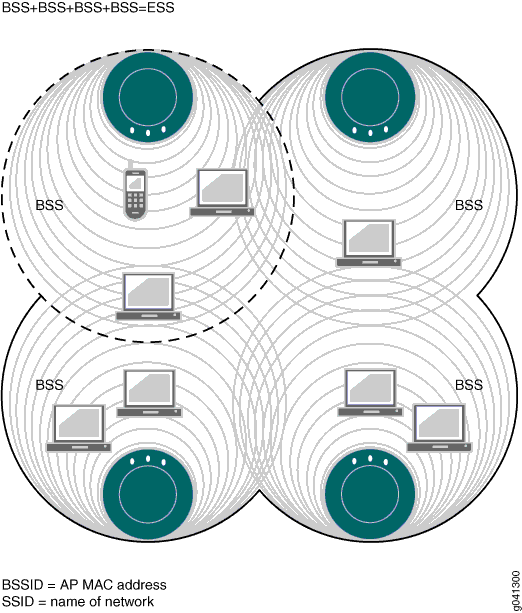
\includegraphics[width=0.8\textwidth]{images/bssssid.png}
	\caption{Jeder Access Point hat eine eigene BSS}
	\label{fig:bssap}
\end{figure}


\section{Verbreitung}
Das Schweizer Bundesamt für Statistik hat im Februar 2011 Daten zur Internetnutzung der Schweiz erhoben und kam zum Schluss, dass 58\% der Schweizer Haushalte über ein Wireless LAN verfügen\citep[S. 8]{bfs.internet.2011}. Zusätzlich werden in den grösseren Städten in den öffentlichen Gebäuden (Bahnhof, Flughafen usw.) sowie in vielen Cafes Wireless LANs Gratis oder gegen Bezahlung angeboten. Zahlen zu der Dichte von Wireless LAN in Europäischen Städten scheint es nicht zu geben oder sind sehr schwierig zu finden. Für die Benutzbarkeit der zu erstellenden App ist das Aufkommen von Wireless LANs in den Städten ein kritischer Faktor.

\subsection{Experiment Zürich}
Um Einschätzen zu können wie viele Access Point in einer Stadt zu finden sind, wurde ein kleines Experiment durch geführt. Mit der Android App WiFi Tracker\citep{google.play.wifitracker} werden alle Wireless LAN Netzwerke in welchen sich das Mobiltelefon befindet, mit den aktuellen GPS Koordinaten gespeichert. Mit dem Fahrrad und dem Mobiltelefon wurde eine Strecke von ca. 3.1 Kilometern durch den Zürcher Kreis 4 abgefahren. Die Aufgezeichneten Daten bringen erstaunliches zum Vorschein.
\begin{figure}[ht]
	\centering
	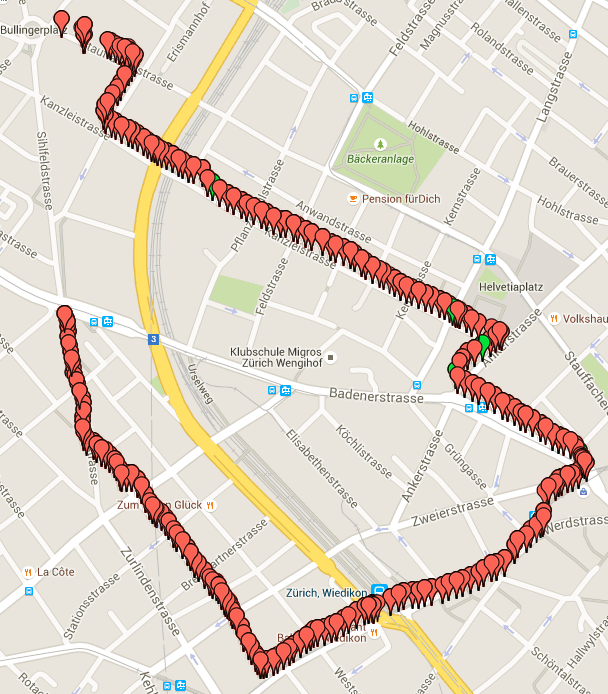
\includegraphics[width=0.8\textwidth]{images/wifikreis4.png}
	\caption{Wireless LANs gemesen mit WiFi Tracker im Zürcher Kreis 4}
	\label{fig:wifikreis4}
\end{figure}
Auf der Strecke wurden 2253 unterschiedliche Access Points gemessen welche in der Abbildung \ref{fig:wifikreis4} visuell dargestellt sind. Das heisst durchschnittlich ist nach 1.37 Meter ein neuer Access Point zu finden. Diese Zahlen müssen natürlich ein wenig relativiert werden da die 2253 Access Points nicht zwingend auch eigene Wireless LAN Netzwerke sind. Wie oben beschrieben können mehrere Access Points mit der selben SSID zu einem Wireless LAN Netzwerk gehören. Zusätzlich ist der Zürcher Kreis 4 nicht ein repräsentatives Gebiet, welches auf den Rest von Zürich oder andere Städte schliessen lässt. Trotzdem lassen diese Zahlen auf eine grosse Wireless LAN Dichte in Schweizerischen Städten deuten.


 % (2. Theoretische Grundlagen)
%!TEX root = ../doc.tex
\chapter{Vorgehen / Methoden}
\label{sec:VorgehenMethoden}

\section{Verwendete Software}
\label{sec:VerwendeteSoftware}
Für die vorliegende Arbeit wurden die unten aufgeführten Programme eingesetzt.

\subsection*{Arbeitsumgebung}\label{wintool}
\begin{itemize}
	\item Microsoft Windows 8 developer preview
\end{itemize}

\subsection*{Virtual Machine}\label{vm}
\begin{itemize}
	\item Oracle VM VirtualBox, Version 3.2.10
\end{itemize}

\subsection*{CAD Catia}\label{catia}
\begin{itemize}
	\item CATIA, Version 5.19 (in VirtualBox)
\end{itemize}

\subsection*{Dokumentation}\label{dokutools}
\begin{itemize}
  \item \LaTeX{} mit TeXnicCenter 2.02 Stable (64 bit)\cite{TeXnicCenter:2014:Online}
	\item proTeXt mit TexMakerX 2.1 (SVN 1774), \href{http://www.latex-project.org/ftp.html}{latex-project.org}
	\item Microsoft Visio 2007
	\item Adobe Acrobat 8 Professional 8.1.6
\end{itemize}
 % Vorgehen / Methoden
%!TEX root = ../doc.tex
\chapter{Use Cases}
\label{sec:usecases}

\begin{usecase}

\addtitle{Use Case 1}{Template test}

%Scope: the system under design
\addfield{Scope:}{System-wide}

%Level: "user-goal" or "subfunction"
\addfield{Level:}{User-goal}

%Primary Actor: Calls on the system to deliver its services.
\addfield{Primary Actor:}{End-User}

%Stakeholders and Interests: Who cares about this use case and what do they want?
\additemizedfield{Stakeholders and Interests:}{
	\item Stakeholder 1 name: his interests
	\item Stakeholder 2 name: his interests
}

%Preconditions: What must be true on start and worth telling the reader?
\addfield{Preconditions:}{}
%when multiple
%\additemizedfield{Preconditions:}{}

%Postconditions: What must be true on successful completion and worth telling the reader
\addfield{Postconditions:}{}
%when multiple
%\additemizedfield{Preconditions:}{}

%Main Success Scenario: A typical, unconditional happy path scenario of success.
\addscenario{Main Success Scenario:}{
	\item The first action
	\item The second action
}

%Extensions: Alternate scenarios of success or failure.
\addscenario{Extensions:}{
	\item[2.a] Invalid login data:
		\begin{enumerate}
		\item[1.] System shows failure message
		\item[2.] User returns to step 1
		\end{enumerate}
	\item[5.a] Invalid subsriber data:
		\begin{enumerate}
		\item[1.] System shows failure message
		\item[2.] User returns to step 2 and corrects the errors
		\end{enumerate}
}

%Special Requirements: Related non-functional requirements.
\additemizedfield{Special Requirements:}{
	\item first applicable non-functional requirement
	\item second applicable non-functional requirement
}

%Technology and Data Variations List: Varying I/O methods and data formats.
\addscenario{Technology and Data Variations List:}{
	\item[1a.] Alternative first action with other technology
}

%Frequency of Occurrence: Influences investigation, testing and timing of implementation.
\addfield{Frequency of Occurrence:}{}

%Miscellaneous: Such as open issues/questions
%\addfield{Open Issues:}{}

\end{usecase}
%!TEX root = ../doc.tex
\chapter{Umsetzung des Prototyps}
\label{sec:umsetzung}

\section{Vorbereitung}

Für die Entwicklung des Prototypen wird Android Studio Version 1.2 von Google verwendet. Android Studio baut auf der freien Version von IntelliJ IDEA auf und verfügt daher über sehr viele nützliche Werkzeuge. Für die Versionskontrolle des Quellecodes wird Git und eine Repository auf Github\footnote{Repository auf Github: \url{https://github.com/roosnic1/wifi_action}} eingesetzt. Für das Testen der App wird ein Android Mobiltelefon des Types Nexus 5 mit der Android Version 5.1 verwendet. Die Dokumentation bzw. der Entwicklerbericht wird in Sublime Text 3 mit \LaTeX{} geschrieben.

\section{Entwicklung}
Für die Umsetzung der App werden im wesentlichen Activities, für die Darstellungen und Interaktionen mit dem Benutzer, sowie ein Receiver und ein Service benötigt. Dazu kommen noch Adapters und Modelle mit welchen Daten in einer Datenbank bzw. in eine Datei serialisiert werden können. Die einzelnen Komponenten werden in diesem Kapitel beschrieben und auf wichtige Eigenschaften wird hingewiesen.

\subsection{Activities}

\subsubsection{MainActivity}
Die MainActivity ist die Ansicht welche dem Benutzer angezeigt wird wenn der Benutzer die App startet. Wie in der Abbildung \ref{fig:mainactivity} beinhaltet die Activity in einer ListView alle bereits erstellten Aktionen und bietet über 2 Buttons die Transaktion zu der LogActivity und ActionActivity an.
\begin{figure}[ht]
	\centering
	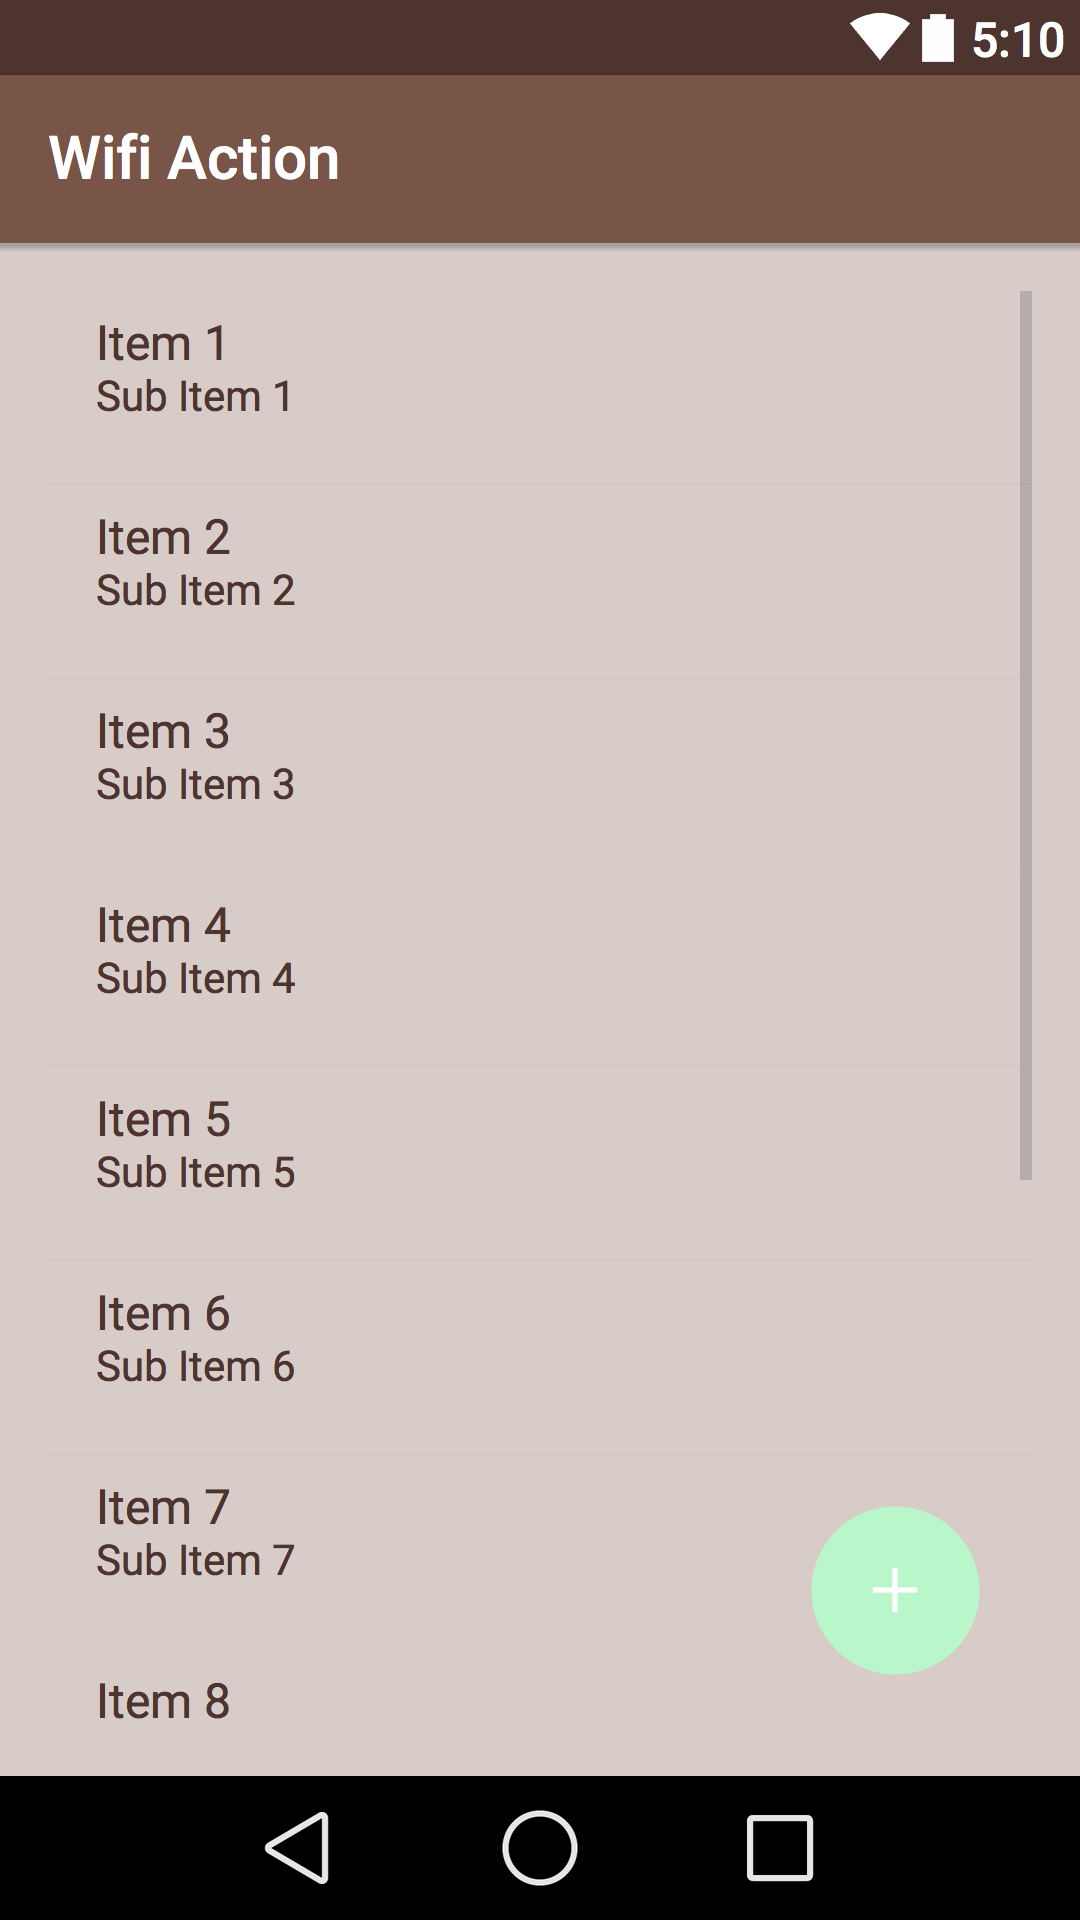
\includegraphics[width=0.4\textwidth]{images/mainactivity.png}
	\caption{Visuelle Repräsentation der MainActivity}
	\label{fig:mainactivity}
\end{figure}
Wenn die MainActivity gestartet wird, wird ein Asynchroner Job gestartet welcher die Serialisierten Aktion aus einer Datei lädt und anzeigt. Beim hinzufügen einer neuen Aktion werden alle Aktionen neu gespeichert damit keine verloren geht. Wenn eine Aktion in der Liste lange geklickt wird, öffnet sich ein Kontext Menu welches das löschen einer Aktion erlaubt. \\
Wird der Plus Button angeklickt werden alle bekannten Wireless LANs geladen und der ActionActivity übergeben. Das Laden der Wireless LANs ist mit Android sehr einfach.
\begin{lstlisting}[language=Java]
	private ArrayList<Wifi> getKnownWifi() {
        WifiManager wifi = (WifiManager) getSystemService(Context.WIFI_SERVICE);
        List<WifiConfiguration> wifis = wifi.getConfiguredNetworks();
        ArrayList<Wifi> wifiList = new ArrayList<>();
        for(WifiConfiguration w : wifis) {
            wifiList.add(new Wifi(w.SSID,w.networkId););
        }
        return wifiList;
    }
\end{lstlisting}
Mit der Funktion getConfiguredNetworks() werden alle Wireless LANs ausgegeben mit denen das Mobiltelefon bereits eine Verbindung hatte.

\subsubsection{ActionActivity}
In der ActionActivity können neue Aktionen eingestellt und gespeichert werden. Im ersten Spinnerelement werden die Verfügbaren Aktionen angezeigt. Je nach Auswahl werden in der restlichen Ansicht unterschiedliche Felder angezeigt oder Versteckt. Deshalb überlagern sich gewisse Elemente in der Abbildung \ref{fig:actionctivity}. Im zweiten Spinnerelement werden die bekannten Wireless LANs angezeigt welche von der MainActivity übergeben wurden. Die restlichen Elemente dienen der Einstellung der Aktion welche über den Button \glqq Save\grqq{} gespeichert werden kann. Bei der Aktion Send SMS besteht die Möglichkeit eine Nummer aus dem Telefonbuch des Androidsystem auszuwählen.
\begin{lstlisting}[language=Java]
    public void onClick(View view) {
        Intent i = new Intent(Intent.ACTION_PICK, ContactsContract.CommonDataKinds.Phone.CONTENT_URI);
        startActivityForResult(i,REQUEST_CONTACTPICKER);
    }

    if(resultCode == RESULT_OK) {
        Uri contentUri = data.getData();
        Cursor cursor = getContentResolver().query(contentUri, null, null, null, null);
        cursor.moveToFirst();
        String number = cursor.getString(cursor.getColumnIndex(ContactsContract.CommonDataKinds.Phone.NUMBER));
        if(number.length() > 0) {
            etMessage3.setText(number);
        }
    }
\end{lstlisting}
Das Telefonbuch wird mit startActivityForResult gestartet und bei der Rückgabe wird der Eintrag aus dem Telefonbuch zurückgeben und ausgewertet. Dies hat den Vorteil dass die App nicht die Berechtigung zum lesen des Telefonbuches benötigt. Beim Drücken des \glqq Save\grqq{} Buttons werden die Daten zusammen gepackt und an die MainActivity zurück gegeben welche die Aktion speichert.
\begin{lstlisting}[language=Java]
-- ActionActivity.java -->
	Action a = new Action(etTitle.getText().toString(),((Wifi)spWifis.getSelectedItem()).getSsid(), at,cbOnConnect.isChecked(),cbOnLeave.isChecked());
	if(mActionType == 0) {
	    a.setStringParam1(etMessage3.getText().toString());
	} else {
	    a.setStringParam1(etMessage1.getText().toString());
	}
	a.setStringParam2(etMessage2.getText().toString());
	a.setBooleanParam1(swBoolean.isChecked());
	Intent i = new Intent();
	i.putExtra("ACTION",a);
	setResult(RESULT_OK, i);
	finish();
<----

-- MainActivity.java -->
	if(resultCode == RESULT_OK) {
		Action a = (Action) data.getSerializableExtra("ACTION");
		mActionList.add(a);
		actionAdapter.notifyDataSetChanged();
		saveActionList();
	}
<----
\end{lstlisting}
\begin{figure}[ht]
	\centering
	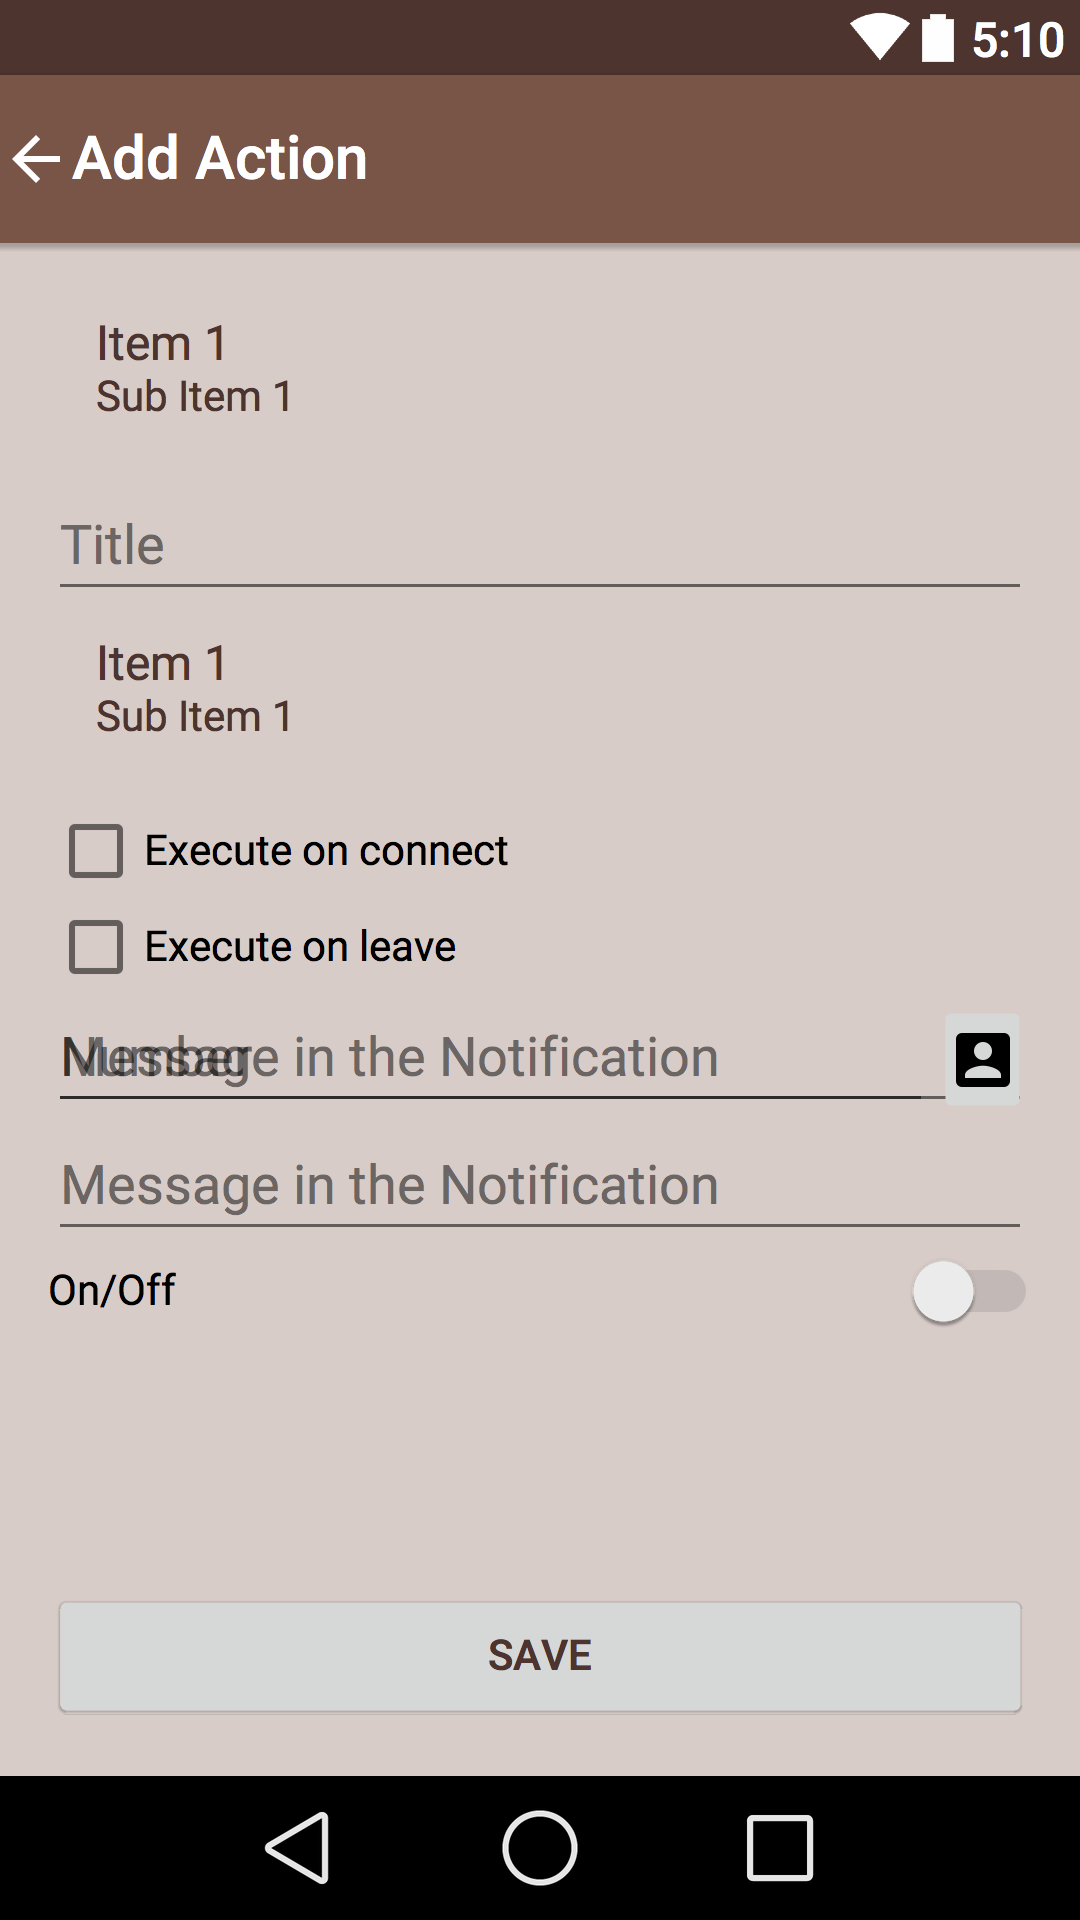
\includegraphics[width=0.4\textwidth]{images/actionactivity.png}
	\caption{Visuelle Repräsentation der ActionActivity}
	\label{fig:actionctivity}
\end{figure}

\subsubsection{LogActivity}
Die LogActivity ist im Vergleich zu den anderen Activities sehr schlicht. Aus einer Datenbank werden alle Log Einträge geladen und angezeigt. Der Adapter der ListView implementiert das VieHolder Prinzip welches auch bei sehr vielen Einträgen ein effizientes und für den Benutzer angenehmes Scrollen durch die Liste erlaubt.

% \begin{figure}[ht]
% 	\centering
% 	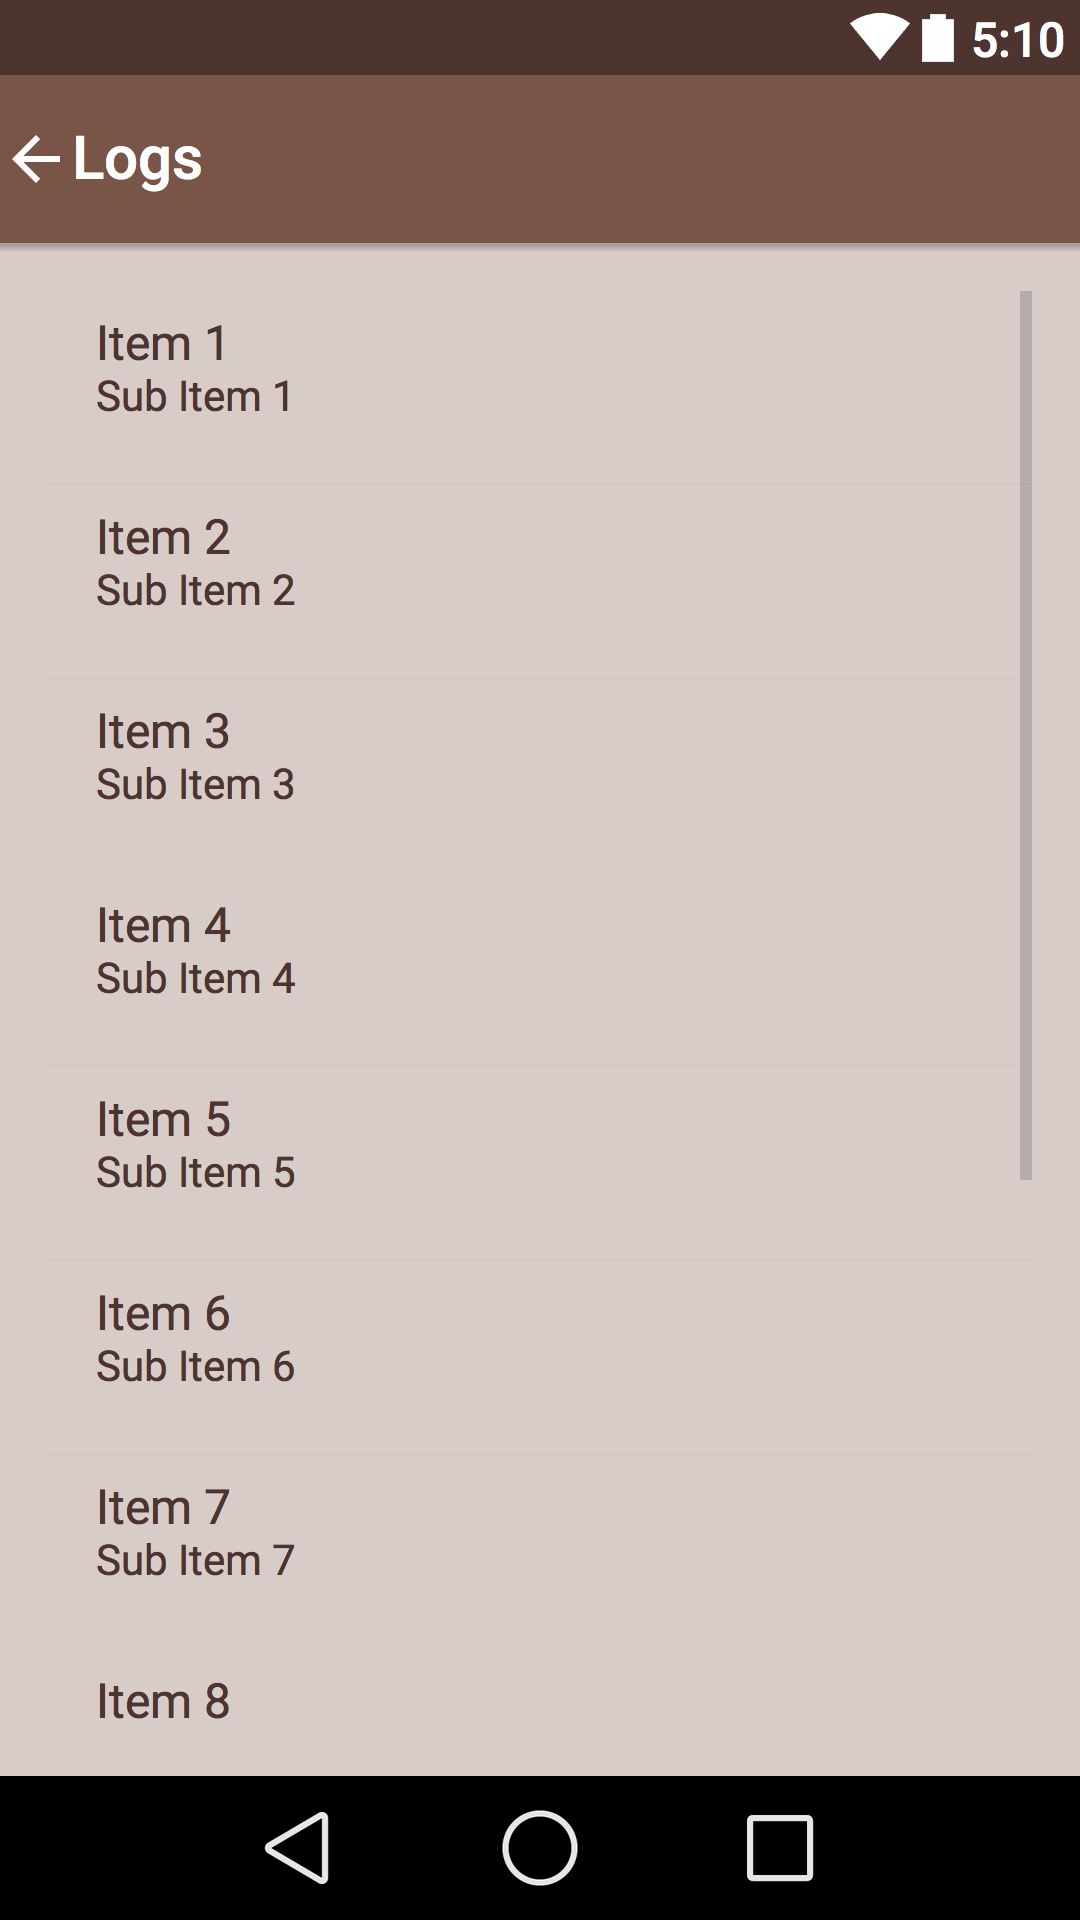
\includegraphics[width=0.4\textwidth]{images/logactivity.png}
% 	\caption{Visuelle Repräsentation der LogActivity}
% 	\label{fig:logactivity}
% \end{figure}

\newpage{}
\subsection{ConnectivityChangedReceiver}
Der ConnectivityChangedReceiver wird aufgerufen wenn es irgendeine Veränderung an der Netzwerkverbindung gibt. Der Receiver muss in der Lage sein zu wissen mit welchem Netzwerk das Mobiltelefon zuvor verbunden bzw. was der Status vor der Änderung der Netzwerkverbindung war. In einer ersten Implementation wurde dies mit Klassen Variabeln gelöst. Die Instanz des ConnectivityChangedReceiver gibt es nur während des Aufrufs und der Ausführung der onReceive Funktion. Darum ging der Wert der Variabeln nach kurzer Zeit Verloren. Die Lösung für dieses Problem heisst Shared Preferences. Mit den Shared Prefrences von Android können der Name und den Status der Netzwerkverbindung persistent gespeichert werden und bei der nächsten Ausführung von onReceive wieder gelesen werden.
\begin{lstlisting}[language=Java]
public void onReceive(Context context, Intent intent) {
    SharedPreferences sharedPreferences = context.getSharedPreferences("com.koki.app.wifiaction",Context.MODE_PRIVATE);
    String currentWifi = sharedPreferences.getString(CW,"");
    String currentState = sharedPreferences.getString(CS,"");
    ConnectivityManager cm = (ConnectivityManager) context.getSystemService(Context.CONNECTIVITY_SERVICE);
    NetworkInfo networkInfo = cm.getActiveNetworkInfo();
    if(networkInfo != null) {
        if(networkInfo.getTypeName().equals(currentState) && networkInfo.getExtraInfo().equals(currentWifi) ) {

        } else if (networkInfo.getTypeName().equals("WIFI") && !networkInfo.getExtraInfo().equals(currentWifi)) {
            ActionService.startAction(context, networkInfo.getExtraInfo(), true);
            sharedPreferences.edit().putString(CW, networkInfo.getExtraInfo()).putString(CS,networkInfo.getTypeName()).commit();
        } else if(currentState.equals("WIFI") && !networkInfo.getTypeName().equals("WIFI")) {
            ActionService.startAction(context, currentWifi, false);
            sharedPreferences.edit().putString(CW,networkInfo.getExtraInfo()).putString(CS,networkInfo.getTypeName()).commit();
        }
    }
}
\end{lstlisting}
In der Funktion onReceive wird überprüft ob der Verbindungstype gewechselt hat oder ob der Wireles LAN Netzwerkname geändert hat und die Funktion im IntentService mit den entsprechenden Parameter aufgerufen.

\subsection{ActionService}

%!TEX root = ../doc.tex
\chapter{Diskussion und Ausblick}
\label{sec:DiskussionUndAusblick}

\textcolor{darkgray}{
  \begin{itemize}
  \item Bespricht die erzielten Ergebnisse bezüglich ihrer Erwartbarkeit, Aussagekraft und Relevanz
  \item Interpretation und Validierung der Resultate
  \item Rückblick auf Aufgabenstellung, erreicht bzw. nicht erreicht
  \item Legt dar, wie an die Resultate (konkret vom Industriepartner oder weiteren Forschungsarbeiten; allgemein) angeschlossen werden kann; legt dar, welche Chancen die Resultate bieten
  \end{itemize}
} % Diskussion und Ausblick

\chapter{Verzeichnisse}
\label{sec:Verzeichnisse}
\addcontentsline{toc}{section}{Literaturverzeichnis}
\bibliography{BibTeX/literatur}
\listoffigures
\addcontentsline{toc}{section}{Abbildungsverzeichnis}
\listoftables
\addcontentsline{toc}{section}{Tabellenverzeichnis}
%!TEX root = ../doc.tex
\chapter*{Glossar}
\label{sec:Glossar}
\addcontentsline{toc}{section}{Abkürzungsverzeichnis}\label{cha:abkürzungsverzeichnis}

In diesem Abschnitt werden Abkürzungen und Begriffe kurz erklärt.
\setglossarystyle{altlistgroup}
\printglossary[title=]


\lstlistoflistings
\addcontentsline{toc}{section}{Listingverzeichnis}

%!TEX root = ../doc.tex
\pagenumbering{Roman}

\appendix
\chapter{Anhang}
\label{sec:Anhang}

\section{Projektmanagement}\label{projektmanagement}

\textcolor{darkgray}{
  \begin{itemize}
  \item Offizielle Aufgabenstellung, Projektauftrag
  \item (Zeitplan)
  \item (Besprechungsprotokolle oder Journals)
  \end{itemize}
}

\section{Weiteres}
\label{sec:Weiteres}

\textcolor{darkgray}{
  \begin{itemize}
  \item CD mit dem vollständigen Bericht als pdf-File inklusive Film- und Fotomaterial
  \item (Schaltpläne und Ablaufschemata)
  \item (Spezifikationen u. Datenblätter der verwendeten Messgeräte und/oder Komponenten)
  \item (Berechnungen, Messwerte, Simulationsresultate)
  \item (Stoffdaten)
  \item (Fehlerrechnungen mit Messunsicherheiten)
  \item (Grafische Darstellungen, Fotos)
  \item (Datenträger mit weiteren Daten (z.B. Software-Komponenten) inkl. Verzeichnis der auf diesem Datenträger abgelegten Dateien)
  \item (Softwarecode)
  \end{itemize}
}


\end{document}
